

\subsection{Synthesis of the HHQ derivative}

The synthesis of HHQ derivative \compound{cmpd:azHHQ} is shown in \ref{sch:azHHQ_synth} and follows a route devised by Baker\cite{Baker2015}. Octanoyl chloride \compound{cmpd:OctoCl} was be converted to $\beta$-Ketoester \compound{cmpd:bke} via a Meldrum's acid adduct\cite{Baker2012,Scribner1978}. The $\beta$-ketoester \compound{cmpd:bke} was condensed with \textit{N}-Boc-\textit{p}-phenylenediamine \compound{cmpd:ambenboc} to form enamine \compound{cmpd:Bocenaman}. The disappointing yield of this step was in part due to the reaction proceeding to an equilibrium state rather than to completion, and hence not all of the starting material being consumed. Starting materials can be recycled to improve the yield. Alternatively, Baker later found a higher-yielding reaction using a \ce{ZrCl4} catalyst.

The enamine \compound{cmpd:Bocenaman} was cyclised with polyphosphoric acid to form amino-HHQ \compound{cmpd:amHHQ} in good yield. The amine group of amino-HHQ \compound{cmpd:amHHQ} was converted to a diazo group by reaction with \ce{NaNO2} and HCl, followed by displacement with \ce{NaN3} to form the final azido-HHQ product \compound{cmpd:azHHQ}\cite{Xu2013}.

\begin{scheme}[H]
	\begin{center}
		\schemeref[Mel]{cmpd:Mel}
		\schemeref[OctoCl]{cmpd:OctoCl}
		\schemeref[bke]{cmpd:bke}
		\schemeref[bket]{cmpd:bket}
		\schemeref[ambenboc]{cmpd:ambenboc}
		\schemeref[Bocenaman]{cmpd:Bocenaman}
		\schemeref[amHHQ]{cmpd:amHHQ}
		\schemeref[azHHQ]{cmpd:azHHQ}
		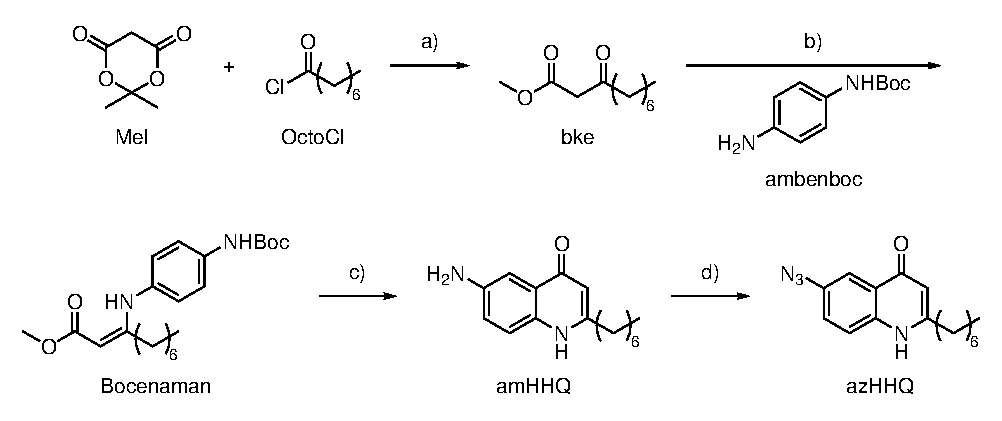
\includegraphics[scale=1]{azHHQ_synth}
		\caption{The synthesis of \compound{cmpd:azHHQ}. 
		a) i) Pyridine, DCM, 0 $^{\circ}$C. ii) MeOH, reflux, 66 \% over two steps. 
		b) MeOH, reflux, 19 \%. 
		c) Polyphosphoric acid, 120 $^{\circ}$C, 72 \%. 
		d) i) \ce{NaNO2}, HCl, \ce{H2O}, 0 $^{\circ}$C. ii) \ce{NaN3}, \ce{H2O}, r.t., 46.5 \%.
		\label{sch:azHHQ_synth}}
	\end{center}
\end{scheme}

%\subsubsection{Retrosynthesis of PQS derivative \compound{cmpd:azPQS}}
%
%The retrosynthesis of PQS derivative \compound{cmpd:azPQS} is shown in \ref{sch:azPQS_retro}. The synthesis of 1-chlorononan-2-one \compound{cmpd:Clnon} from heptyl magnesium bromide \compound{cmpd:hepGr}\cite{Hodgkinson2012} and the Weinreb amide \compound{cmpd:ClWa}\cite{Hodgkinson2011} prepared from chloroacetyl chloride \compound{cmpd:ClAcCl} has been previously described by Hodgkinson \textit{et al.}\cite{Hodgkinson2012}. 
%The synthesis of PQS described by Hodgkinson \textit{et al.}\cite{Hodgkinson2012} uses a microwave reaction of 1-chlorononan-2-one \compound{cmpd:Clnon} with anthranilic acid. It was hoped that the azide group could be installed by using 5-nitroanthranilic acid \compound{cmpd:5naa} in the place of anthranilic acid in this microwave reaction, so that the nitro group could then be converted to an azide group via an amine. However, the microwave-catalysed reaction fails when 5-nitroanthranilic acid \compound{cmpd:5naa} is used\cite{Baker2014}. Therefore, a two step process is employed instead. Firstly, ester \compound{cmpd:5naae} is formed by S$_N$2 displacement of the chlorine atom of 1-chlorononan-2-one \compound{cmpd:Clnon} by the carboxylate group of 5-nitroanthranilic \compound{cmpd:5naa}. The ester \compound{cmpd:5naae} is then cyclised using a polyphosphoric acid-catalysed reaction developed by Hradil \textit{et al.}\cite{Hradil1999} to form nitro-PQS \compound{cmpd:NPQS}.
%The nitro group can then be hydrogenated to form amino-PQS \compound{cmpd:amPQS} followed by conversion to azido-PQS \compound{cmpd:azPQS}\cite{Xu2013}.
%
%
%\begin{scheme}[H]
%	\begin{center}
%		\schemeref[hepBr]{cmpd:hepBr}
%		\schemeref[hepGr]{cmpd:hepGr}
%		\schemeref[ClAcCl]{cmpd:ClAcCl}
%		\schemeref[ClWa]{cmpd:ClWa}
%		\schemeref[Clnon]{cmpd:Clnon}
%		\schemeref[5naa]{cmpd:5naa}
%		\schemeref[5naae]{cmpd:5naae}
%		\schemeref[NPQS]{cmpd:NPQS}
%		\schemeref[amPQS]{cmpd:amPQS}
%		\schemeref[azPQS]{cmpd:azPQS}
%		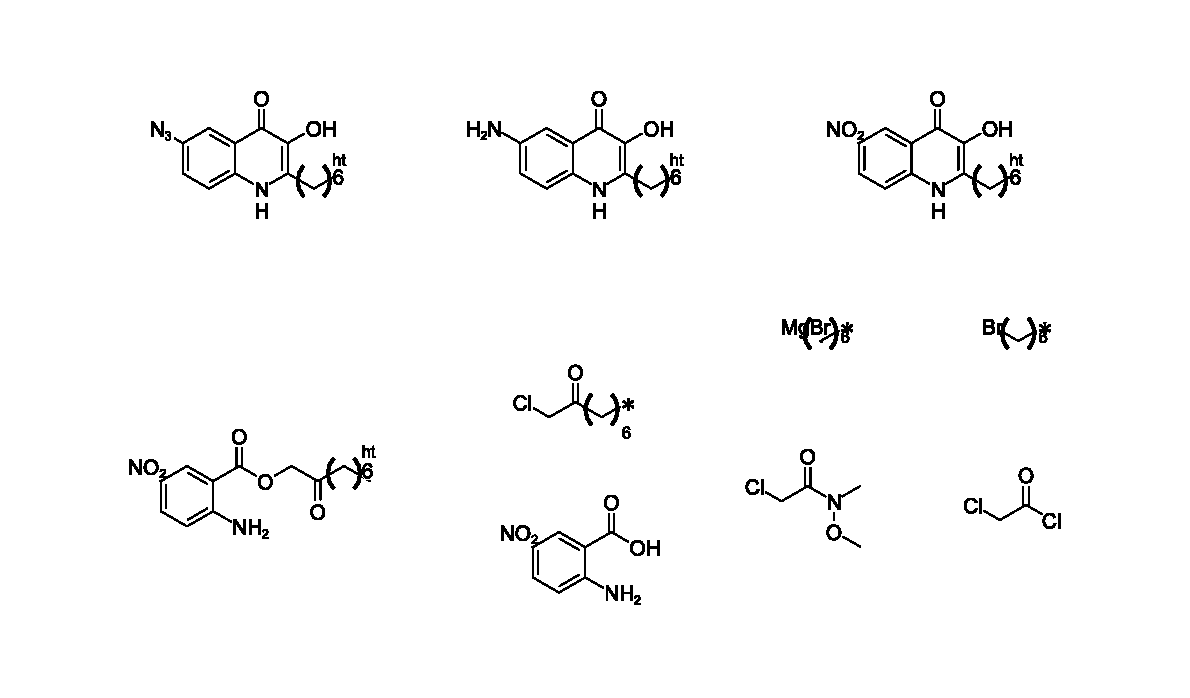
\includegraphics[scale=1]{azPQS_retro}
%		\caption{The retrosynthesis of PQS derivative \compound{cmpd:azPQS}. \label{sch:azPQS_retro}}
%	\end{center}
%\end{scheme}

\subsection{Synthesis of the PQS derivative \compound{cmpd:azPQS}}

The synthesis of PQS derivative \compound{cmpd:azPQS} is shown in \ref{sch:azPQS_synth}, and also follows a route devised by Baker\cite{Baker2015}.The Weinreb amide \compound{cmpd:ClWa}\cite{Hodgkinson2011} was prepared from chloroacetyl chloride, followed by attack with heptyl magnesium bromide \compound{cmpd:hepGr} to form 1-chlorononan-2-one \compound{cmpd:Clnon} following a procedure described by Hodgkinson \textit{et al.}\cite{Hodgkinson2012}. 

The synthesis of PQS described by Hodgkinson \textit{et al.}\cite{Hodgkinson2012} uses a microwave reaction of 1-chlorononan-2-one \compound{cmpd:Clnon} with anthranilic acid. It was hoped that the azide group could be installed by using 5-nitroanthranilic acid \compound{cmpd:5naa} in the place of anthranilic acid in this microwave reaction, so that the nitro group could then be converted to an azide group via an amine. However, the microwave-catalysed reaction fails when 5-nitroanthranilic acid \compound{cmpd:5naa} is used\cite{Baker2015}. Therefore, a two step process was employed instead. 

5-Nitroanthranilic acid \compound{cmpd:5naa} was heated with \ce{K2CO3} to deprotonate the carboxylic acid, followed by addition of 1-chlorononan-2-one \compound{cmpd:Clnon} to form the ester \compound{cmpd:5naae} by S$_N$2 displacement of the chlorine atom in a procedure adapted from Hlav\'a\u c \textit{et al.}\cite{Hlavac2004}. Cyclisation with polyphosphoric acid produced nitro-PQS \compound{cmpd:NPQS} cleanly\cite{Hlavac2004,Hradil1999}. 

Conditions for the reduction of the nitro group were then compared (see \ref{tbl:amPQS_opt}). Baker initially used Zn and HCl, however this gave a yield over 100 \% suggesting coordination of Zn to the amino-PQS \compound{cmpd:amPQS}\cite{Baker2015} (this product was taken through and purified after the next step). She also attempted reduction with Pd/C and \ce{H2} or ammonium formate, but no reaction was observed.

Further conditions were tested in this work in order to obtain a clean sample of amino-PQS \compound{cmpd:amPQS}.
An initial test of reduction with \ce{SnCl2} produced no detectable product by LCMS. 
Catalytic hydrogenation using harsher conditions was then attempted, and it was determined that increasing the pressure to 3 atm using a Paar hydrogenator causes full conversion in 4 h using Pd/C and \ce{H2}. 
Good yields (80 \%) were also achieved using \ce{PtO2} as a catalyst, with the advantage that the reaction proceeds more quickly, and at atmospheric pressure and temperature\cite{Shen2006a}. 

Finally, amino-PQS \compound{cmpd:amPQS} was converted to azido-PQS \compound{cmpd:azPQS} by reaction with \ce{NaNO2} and HCl to form diazo-PQS, followed by displacement of the diazo group using \ce{NaN3} to give the azido-PQS \compound{cmpd:azPQS}\cite{Xu2013}. The yield of this reaction was rather disappointing (28 \%), and is probably due to loss of product in the supernatant following precipitation\cite{Baker2015}.

\renewcommand{\arraystretch}{1.2}
\begin{table}[ht]
  \centering
\begin{tabular}{|l|l|}
\hline 
\textbf{Conditions} & \textbf{Outcome} \\ 
\hline 
\ce{H2}, Pd/C, 1 atm, r.t., 18 h & No reaction\cite{Baker2015} \\ 
\hline 
\ce{NH4HCO2}, Pd/C, 1 atm, r.t., 18 h & No reaction\cite{Baker2015} \\ 
\hline 
Zn, HCl (aq), r.t., 5 min h & Product \compound{cmpd:amPQS} + Zn, assumed quantitative yield\cite{Baker2015} \\ 
\hline 
\ce{SnCl2}.2\ce{H2O}, MeOH, r.t., 18 h & No reaction \\ 
\hline 
\ce{H2}, Pd/C, MeOH, 3 atm, r.t., 4 h. & Product \compound{cmpd:amPQS}, 100 \% yield \\ 
\hline 
\ce{H2}, \ce{PtO2}, MeOH, 1 atm, r.t., 45 min & Product \compound{cmpd:amPQS}, 80 \% yield \\ 
\hline 
\end{tabular}
\caption{Conditions attempted for the synthesis of \compound{cmpd:amPQS}. \label{tbl:amPQS_opt}} 
\end{table}

\begin{scheme}[H]
	\begin{center}
		\schemeref[hepBr]{cmpd:hepBr}
		\schemeref[hepGr]{cmpd:hepGr}
		\schemeref[ClAcCl]{cmpd:Cl2Cl}
		\schemeref[ClWa]{cmpd:ClWa}
		\schemeref[Clnon]{cmpd:Clnon}
		\schemeref[5naa]{cmpd:5naa}
		\schemeref[5naae]{cmpd:5naae}
		\schemeref[NPQS]{cmpd:NPQS}
		\schemeref[amPQS]{cmpd:amPQS}
		\schemeref[azPQS]{cmpd:azPQS}
		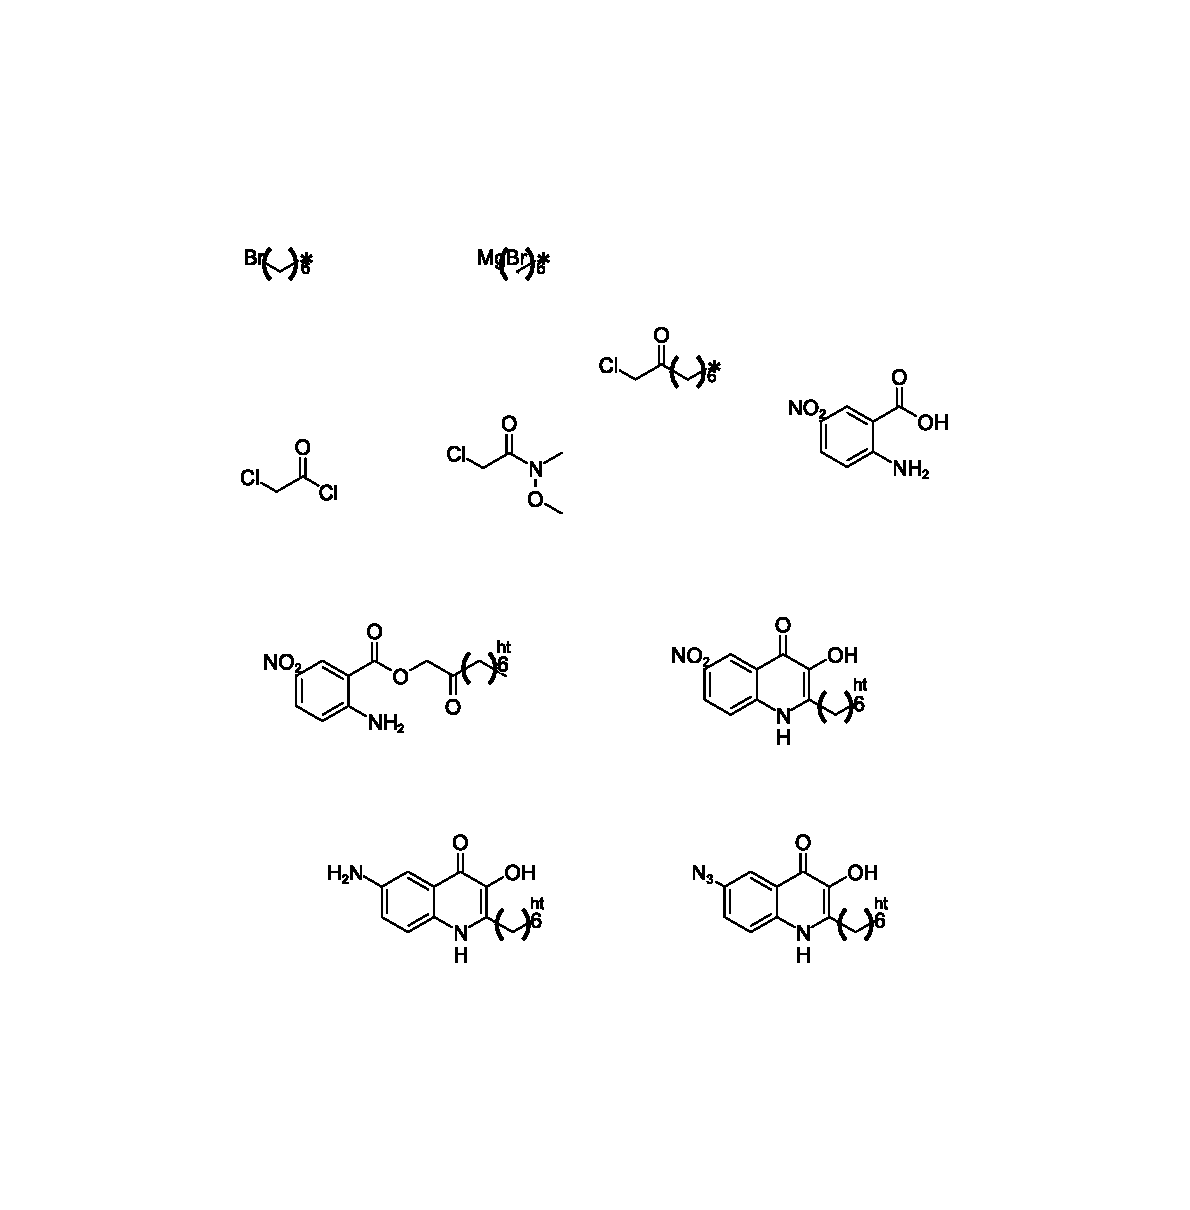
\includegraphics[scale=1]{azPQS_synth}
		\caption{The synthesis of \compound{cmpd:azPQS}.
		a) Mg turnings, THF, r.t., 2 h then reflux, 2 h.
		b) \textit{N},\textit{O}-dimethylhydroxyl amine hydrochloride, \ce{K2CO3}, toluene, \ce{H2O}, - 5 $^{\circ}$C to r.t., 30 min, 71 \%.
		c) THF, 0 $^{\circ}$C to r.t., 15 h, 96 \%.
		d) \compound{cmpd:5naa}, \ce{K2CO3}, DMF, 90 $^{\circ}$C, 1 h, then \compound{cmpd:Clnon}, r.t., 18 h, 100 \%.
		e) Polyphosphoric acid, 90 $^{\circ}$C, 5.5 h, 40 \%.
		f) \ce{H2}, \ce{PtO2}, MeOH, 1 atm, r.t., 45 min, 80 \%.
		g) i) \ce{NaNO2}, HCl, \ce{H2O}, 0 $^{\circ}$C, 50 min. ii) \ce{NaN3}, \ce{H2O}, r.t., 4 h, 28 \% over two steps.
		\label{sch:azPQS_synth}}
	\end{center}
\end{scheme}

\subsection{Synthesis of C$_4$-HSL derivatives\label{sec:HSLs}}

N$_3$-C$_2$-HSL \compound{cmpd:HL2N3} (the azido derivative of C$_4$-HSL with a C$_2$ chain, see \ref{sch:HL2N3_synth}) has previously been prepared by Stacy \textit{et al.} \cite{Stacy2013}. Their synthesis was followed, starting with the cyclisation of \textsc{l}-methionine \compound{cmpd:LM} using bromoacetic acid to form the homoserine lactone HBr salt \compound{cmpd:HLHBr}. The disappointing yield can be attributed to difficulties in precipitating the final product. The homoserine lactone HBr salt \compound{cmpd:HLHBr} was then converted by a biphasic one-pot process to N$_3$-C$_2$-HSL \compound{cmpd:HL2N3} using bromoacetyl bromide \compound{cmpd:Br2Br} and \ce{NaN3}. 

\begin{scheme}[H]
	\begin{center}
		\schemeref[LM]{cmpd:LM}
		\schemeref[HLHBr]{cmpd:HLHBr}
		\schemeref[Br2Br]{cmpd:Br2Br}
		\schemeref[HL2N3]{cmpd:HL2N3}
		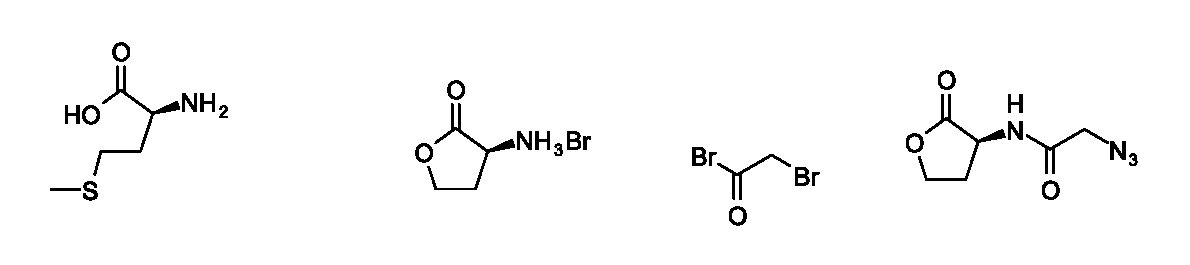
\includegraphics[scale=1]{HL2N3_synth}
		\caption{The synthesis of \compound{cmpd:HL2N3}.
		a) Bromoacetic acid, \textit{i}-PrOH:\ce{H2O}:AcOH (5:5:2), r.t., 18 h, 41 \%.
		b) \ce{NaN3}, \ce{NaHCO3}, \ce{H2O}/\ce{CH2Cl2}, r.t., 18 h, 41 \%.
		\label{sch:HL2N3_synth}}
	\end{center}
\end{scheme}

It was hoped that this procedure could also be used to produce the C$_4$ and C$_6$ derivatives, however, attempts to convert homoserine lactone \compound{cmpd:LM} to N$_3$-C$_4$-HSL \compound{cmpd:HL4N3} using 4-bromobutyryl chloride \compound{cmpd:Cl4Br} produced a complex mixture of products. This is likely to be because the S$_N$2 reaction in which the azide anion displaces bromine is slower for the C$_4$ derivative as the bromine atom being displaced is no longer adjacent to a carbonyl group. In addition, the longer chain length allows intramolecular cyclisation of the bromide with the secondary amide. 
The conversion was therefore carried out as a two-step process, where a bromoacyl chain was initially installed, followed by the S$_N$2 reaction with \ce{NaN3} (see \ref{sch:HL46N3_synth}). 

Reaction of the homoserine lactone HBr salt \compound{cmpd:HLHBr} with 4-bromobutyryl chloride \compound{cmpd:Cl4Br} or 6-bromohexanoyl chloride \compound{cmpd:Cl6Br} produced Br-C$_4$-HSL \compound{cmpd:HL4Br} or Br-C$_6$-HSL \compound{cmpd:HL6Br} respectively, in good yields. Heating with \ce{NaN3} in DMF converted Br-C$_6$-HSL \compound{cmpd:HL6Br} to N$_3$-C$_6$-HSL \compound{cmpd:HL6N3}. 
Similar conditions were used by Dr. Bin Yu, a visiting PhD student in the Spring group, to convert the bromo-C$_4$ derivative \compound{cmpd:HL4Br} to the azido-C$_4$ derivative \compound{cmpd:HL4N3}, and this compound was kindly donated to complete the set. 
Yields for the S$_N$2 reaction could probably be improved by decreasing the temperature (see \ref{sch:SHL4CipMe_synth}, for example).

\begin{scheme}[H]
	\begin{center}
		\schemeref[LM]{cmpd:LM}
		\schemeref[HLHBr]{cmpd:HLHBr}
		\schemeref[Cl4Br]{cmpd:Cl4Br}
		\schemeref[Cl6Br]{cmpd:Cl6Br}
		\schemeref[HL4Br]{cmpd:HL4Br}
		\schemeref[HL6Br]{cmpd:HL6Br}
		\schemeref[HL4N3]{cmpd:HL4N3}
		\schemeref[HL6N3]{cmpd:HL6N3}
		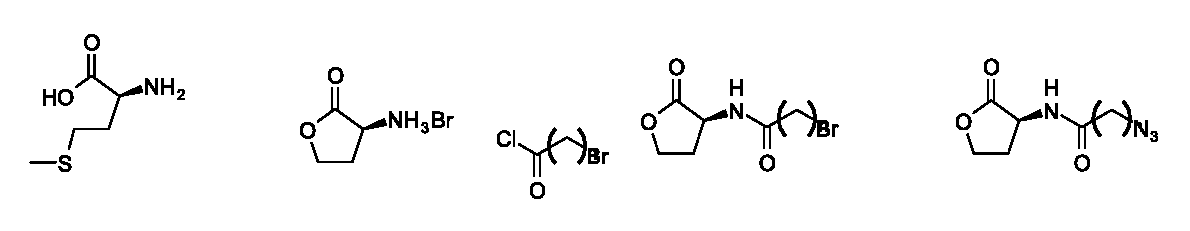
\includegraphics[scale=1]{HL46N3_synth}
		\caption{The synthesis of \compound{cmpd:HL4N3} and \compound{cmpd:HL6N3}.
		a) Bromoacetic acid, \textit{i}-PrOH:\ce{H2O}:AcOH (5:5:2), r.t, 18 h, 41 \%.
		b) \ce{NaHCO3}, \ce{H2O}/\ce{CH2Cl2}, r.t., 18 h, \compound{cmpd:HL4Br}: 80 \%, \compound{cmpd:HL6Br}: 66 \%.
		c) \ce{NaN3}, DMF, 100 $^{\circ}$C, 5 h,\compound{cmpd:HL6N3}: 27 \% (donated by Dr. Bin Yu), \compound{cmpd:HL6N3}: 56 \%.
		\label{sch:HL46N3_synth}}
	\end{center}
\end{scheme}